\documentclass[../../../main.tex]{subfiles}
 
\begin{document}

In reflecting on my advising practices with my STEM students, I realize that there is an implicit decision-tree that lives in my mind (see Fig. \ref{fig:tree}).  I use this decision-tree to guide students in LinkedIn profile creation, resume-writing, and writing letters of recommendation\footnote{Examples of letters of recommendation for a variety of students are included in the supporting materials.}.  \textit{It is important to note that Fig. \ref{fig:tree} does not represent any sort of hierarchy, but merely the order in which I proceed with the students.}  Reflecting on my conversations with the students reveals that the discernment process simply follows this pattern.  Practical concerns about potential salary, proximity to family, and technical ability all factor into the path of the student through the process described by Fig. \ref{fig:tree}.

\begin{figure}
\centering
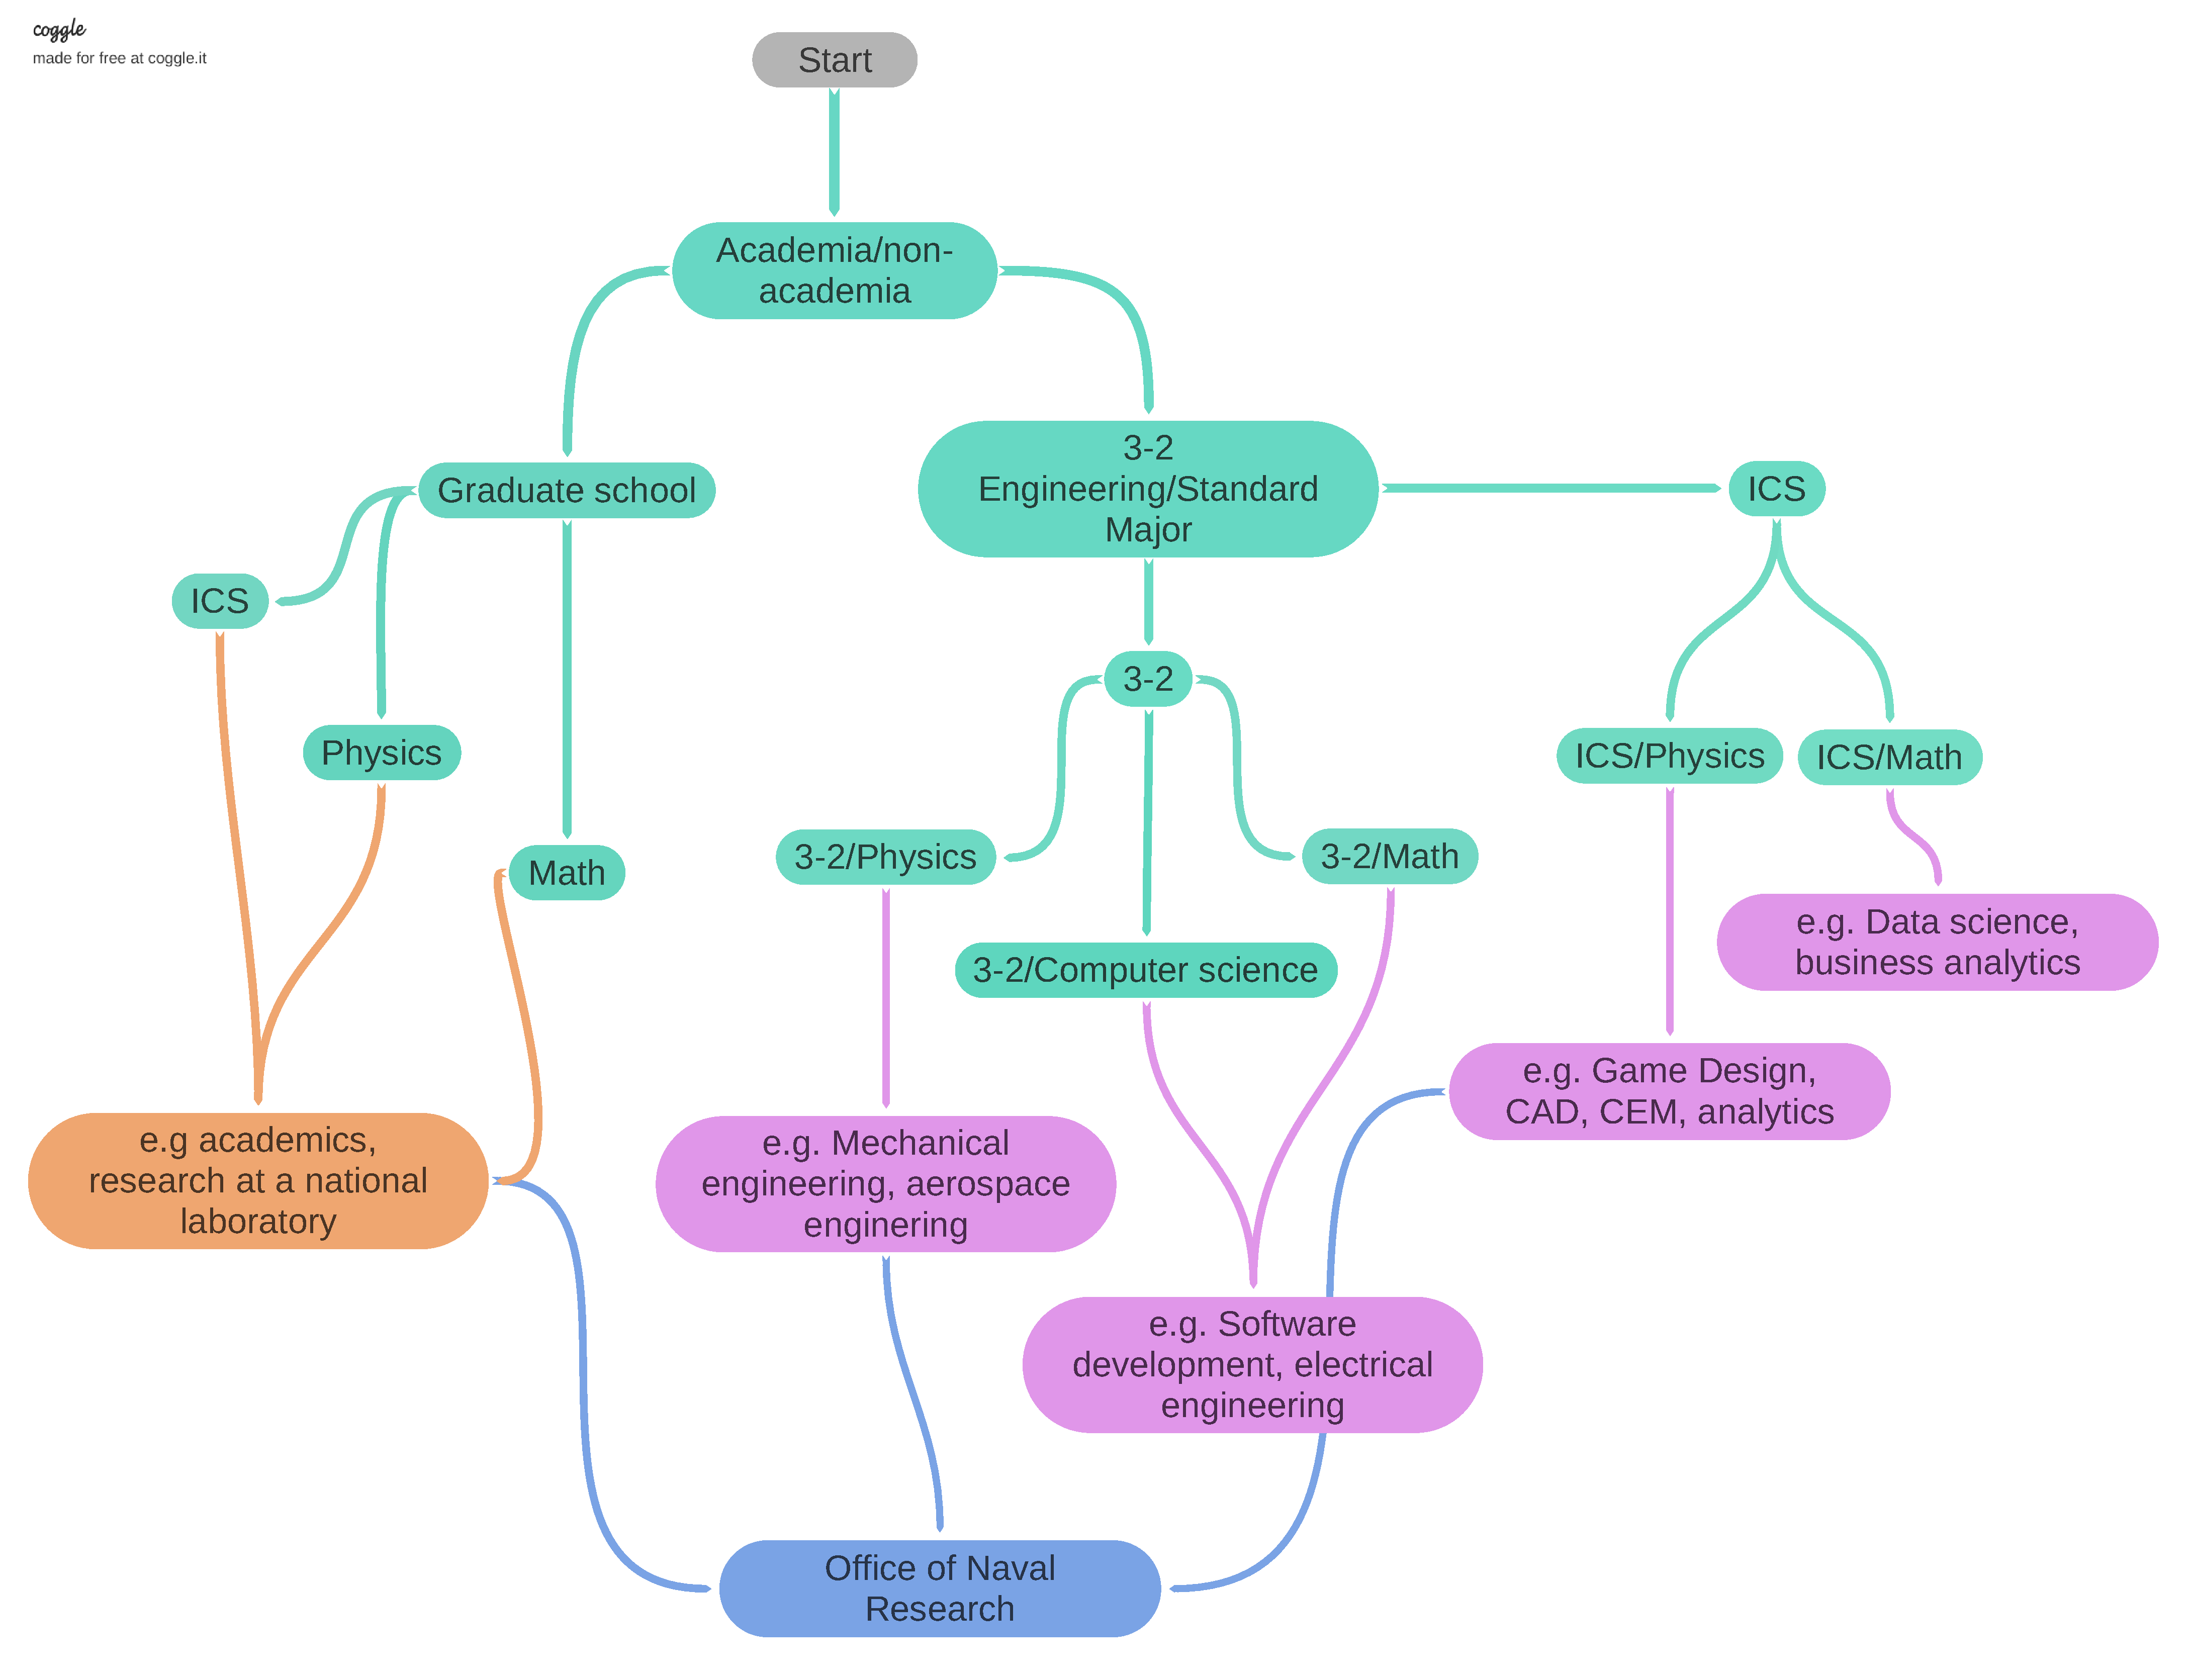
\includegraphics[width=0.75\textwidth]{figures/Advising_tree.pdf}
\caption{\label{fig:tree} A decision-tree that orders my thinking around the advising of my STEM students.}
\end{figure}

\subsection{Discernment within STEM: Major Selection, and Diverse Pathways to Graduation}

\textit{Discernment} means the ability to understand oneself, while seeking honest guidance to make one more spiritually and mentally sound.  Advising STEM majors sometimes requires me to provide them a form of ``professional candor'' that the FPC is tasked with providing me.  If we do not identify where we need to grow, then we are either not hearing the guidance given by peers, or not adequately reflecting on our situation.  This was the case when one of my first year students, Wyatt, shared with me that he wanted to study physics.  He shared with me that he was not keen on taking calculus, and did not find his computer science course exciting.  This was a clue to me that he was not on the right track.  Normally, a physics student would sink his or her teeth into these courses.  After a period of discernment in Spring 2021, we found that Wyatt was not interested in physics because of the \textit{scientific experimentation} portion of it.  He was interested in physics because he liked understanding and playing with the way the world fits together in his mind.  Given his interest in manga and anime, I recommended he talk to his family about digital art and design.  I also noted that Whittier College offers courses in world building and graphical design.
\\
\vspace{0.25cm}
Sometimes students arrive in my office already having discerned that they want to make a career in science.  At the first decision point, we have \textit{academia or non-academia.}  This decision is usually the first decision, because the course list our department requires for the academic track in physics contains more theoretical physics and math courses.  Usually, if the student wants to attend graduate school, they have discerned that as well.  The real task in that case is to discern which area of academia they wish to explore.  Since we now require COSC120, Computer Science I, for physics majors, students can experience computer science before deciding between ICS or PHYS as a major track.  Although I have taught and mentored students who were straight mathematics majors, none of them were my advisees.  During the middle of the junior year, we begin the graduate school search and application-building process.  If there is an academic connection to my CEM/ONR research, we can explore potential connections in their senior projects if the student desires.
\\
\vspace{0.25cm}
On the other side of the decision point, there is the private or public-sector path.  In Fig. \ref{fig:tree}, the rest of the decision tree branches into the different topics and example career selections.  Common private sector career selections involve CAD design for engineering firms and software development for gaming companies.  The decision regarding 3-2 program versus ICS needs to be made during the first or second semester in order to plan the student's courses.  Once I see a committment to the 3-2 program, I help the student plan their courses for every semester.  Though the 3-2 majors do not complete a senior project, I involve them in my CEM/ONR research if possible during the summers.  This is so they can gain the experience necessary to secure valuable internships and projects at their next institution (usually USC).
\\
\vspace{0.25cm}
If the student wants to be at Whittier for four years, but not major in physics, the choice is usually ICS/Physics or ICS/Math.  A growing career selection for this area is data science, and we are now offering two new courses in data science at Whittier College.  One trick I have added to my LinkedIn advising lately is the geographical job search.  Because there are so many firms in Southern California that specialize in data science, the student and I generate some search terms and then run a geographical search within LinkedIn for matches.  We narrow the field by eliminating the organizations that are located too far from the family of the student.  The search radius is their choice, of course.  I find this is a useful way to gauge the extent to which a student will go to secure a role at such firms.  The narrowed list of firms provides the students with example jobs they can peruse for skill requirements.  Finally, we think about ways in which final projects and course selections connect to the skill requirements.  This was especially important for Matthew Buchanan Garza, one of my advisees, who wants to enter the world of software design for gaming.  Knowing that algorithm development is highly important for software development and gaming roles, we prioritized the corresponding course in his schedule.  The job search also provides a variety of sound choices, rather than winning the lottery by applying to Blizzard or Rockstar alone.

\end{document}
